\section{Basic Tutorials 2}

%%%%%%%%%%%%%
\subsection{Filters}

%% Break
\begin{frame}{Basic Tutorial 2}
\fontsize{36pt}{36pt}\selectfont
\center
\begin{center}
Basic Tutorial 2
\end{center}
\end{frame}

\begin{frame}{Note on the Tutorial}
\begin{itemize}
  \item Most examples will be Python
  \item Obvious translation to other languages
  \item C++ usage (generally) obvious
\end{itemize}
\end{frame}

\subsection{Example}
\begin{frame}{Hands On}
\fontsize{36pt}{36pt}\selectfont
\center
\begin{center}
Hands On
\end{center}
\vspace{20pt}
\begin{center}
\fontsize{11pt}{11pt}\selectfont
\texttt{Examples/BasicTutorial2/Filters.py}
\end{center}
\end{frame}

\begin{frame}[fragile]
\frametitle{What just happened?}
\lstpython
\begin{lstlisting}
# Simple smoothing
smooth = sitk.SmoothingRecursiveGaussian ( image, 2.0 )
sitk.Show ( sitk.Subtract ( image, smooth ) )
...
RuntimeError: Exception thrown in SimpleITK Subtract: ...
sitk::ERROR: Both images for SubtractImageFilter don't match type or dimension!
...
\end{lstlisting}

\begin{itemize}
  \item The output of SmoothingRecursiveGaussian is of type float
  \item The input image is signed short
  \item Most SimpleITK filters with 2 inputs require the same type
  \item Let's fix the problem
\end{itemize}

\end{frame}

\begin{frame}[fragile]
\frametitle{Introducing Cast}
\lstpython
\begin{lstlisting}
# Much better
print "Before: ", smooth.GetPixelIDTypeAsString()
smooth = sitk.Cast ( smooth, image.GetPixelIDValue() )
print "After: ", smooth.GetPixelIDTypeAsString()
sitk.Show ( sitk.Subtract ( image, smooth ), "DiffWithGaussian" )
\end{lstlisting}
Back to iPython (\texttt{Examples/BasicTutorial2/Filters.py})
\end{frame}


\begin{frame}[fragile]
\frametitle{Sizes and Indices}
\lstpython
\begin{lstlisting}
# Extract
size = [64, 64, 1]
start = [64, 0, 0]
sitk.Show ( sitk.Extract ( image, size, start ), "Extracted" )
\end{lstlisting}
in C++ / ITK code this would use
\lstcpp
\begin{lstlisting}
typedef unsigned char PixelType;
enum {ImageDimension = 2};
typedef itk::Image<PixelType,ImageDimension> ImageType;

typedef ImageType::IndexType  IndexType;
typedef ImageType::SizeType   SizeType;
typedef ImageType::RegionType RegionType;
\end{lstlisting}
\begin{itemize}
\item SimpleITK uses STL vectors
\item Wrapping converts to language-specific constructs (tuples/arrays)
\end{itemize}
\end{frame}


%% Morphology
\subsection{Morphology}

\begin{frame}{Morphology}
\fontsize{36pt}{36pt}\selectfont
\center
\begin{center}
Morphology
\end{center}
\vspace{20pt}
\begin{center}
\fontsize{11pt}{11pt}\selectfont
\texttt{Examples/BasicTutorial2/Morphology.py}
\end{center}
\end{frame}

\begin{frame}[fragile]
\frametitle{Operators}

\begin{columns}[c]

\column{0.25\textwidth}
\begin{center}
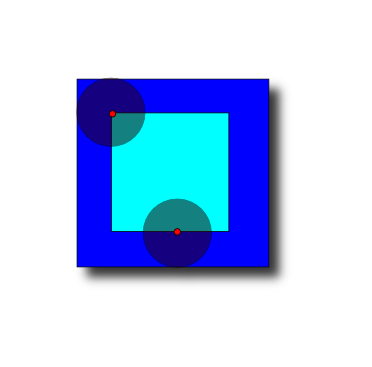
\includegraphics[width=1\textwidth]{Images/Erosion_shadow} \\
Erosion
\end{center}

\column{0.25\textwidth}
\begin{center}
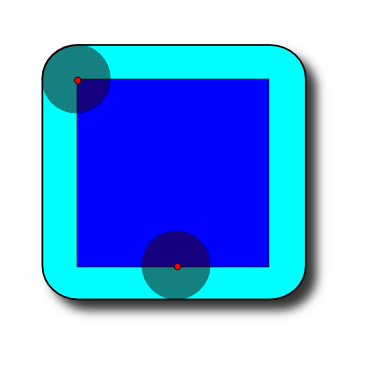
\includegraphics[width=1\textwidth]{Images/Dilation_shadow} \\
Dilation
\end{center}

\column{0.25\textwidth}
\begin{center}
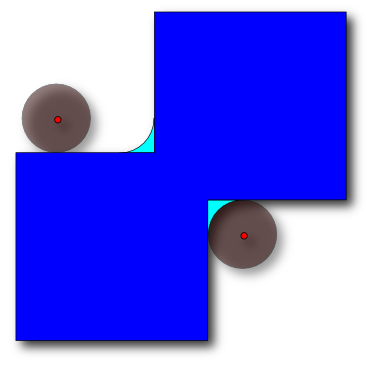
\includegraphics[width=1\textwidth]{Images/Closing_shadow} \\
Closing
\end{center}

\column{0.25\textwidth}
\begin{center}
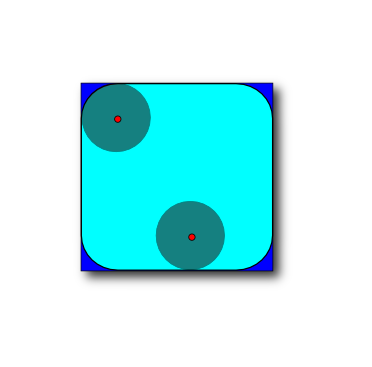
\includegraphics[width=1\textwidth]{Images/Opening_shadow} \\
Opening
\end{center}
\end{columns}
\vspace{12pt}
Images from \url{http://en.wikipedia.org/wiki/Mathematical_morphology}
\end{frame}

\begin{frame}{Morphology in Action}
\center
\begin{center}
Back to iPython (\texttt{Examples/BasicTutorial2/Morphology.py})
\end{center}
\end{frame}

\begin{frame}[fragile]
\lstpython
\begin{lstlisting}
# Use pixel-wise operators
sitk.Show ( 127 * image + 127 * sitk.BinaryErode ( image ), "ThinErosion" )
\end{lstlisting}
\frametitle{Pixel-wise Operators}
\begin{threeparttable}
  \caption{SimpleITK Pixel-wise Operators}
  \begin{tabular}{c||l|l}
    Operator & Equivalant & Usage\tnote{$^\dagger$} \\
    \hline
    $+$        & Add, AddConstantTo & $A + B$, $s+A$, $s+B$ \\
    $-$        & Subtract, SubtractConstantFrom & $A - B$, $s-A$, $s-B$ \\
    $*$        & Multiply, MultiplyByConstant & $A * B$, $s*A$, $s*B$ \\
    $/$        & Divide, DivideByConstant & $A / B$, $s/A$, $B/s$ \\
    $\&$        & And ``and'' & $A \& B$ \\
    $|$        & Or ``or'' & $A | B$ \\
    $\sim$        & Not ``not'' & $~A$
  \end{tabular}
  \begin{tablenotes}
    \item[$^\dagger$] $A$ and $B$ are images (2D or 3D), $s$ is a scalar
  \end{tablenotes}
\end{threeparttable}
\end{frame}

\begin{frame}[fragile]
\frametitle{Operator Example}
\lstpython
\begin{lstlisting}
sitk.Hash ( image + 2 )
sitk.Hash ( sitk.AddConstantTo ( image, 2 ) )

sitk.Hash ( image * 2 )
sitk.Hash ( sitk.MultiplyByConstant ( image, 2 ) )
\end{lstlisting}

\begin{itemize}
  \item Hash calculates the MD5 or SHA1 hash of the \textit{image} data
  \item Used to tell if two images are exactly identical
\end{itemize}
Back to iPython (\texttt{Examples/BasicTutorial2/Morphology.py})
\end{frame}


%% \subsection{Label Maps}

%% %% Label maps
%% \begin{frame}{Label Maps}
%% \fontsize{36pt}{36pt}\selectfont
%% \center
%% \begin{center}
%% Label Maps
%% \end{center}
%% \end{frame}

%% Break
\begin{frame}{Break}
\fontsize{36pt}{36pt}\selectfont
\center
\begin{center}
Let's take a break
\end{center}
\end{frame}

